\title{Tendon Robot Dynamics}
\author{John Till}
\date{}

\documentclass[12pt]{article}

\usepackage[a4paper, margin=0.75in]{geometry}
\usepackage[colorlinks=true,urlcolor=blue]{hyperref}
\usepackage{amsmath,amssymb}
\usepackage{graphicx}

\usepackage{xcolor}
\definecolor{OffWhite}{rgb}{0.93,0.93,0.93}
\definecolor{QtCommentColor}{rgb}{0,0.5,0}
\definecolor{QtKeywordColor}{rgb}{0.5,0.5,0}
\definecolor{QtPurpleColor}{rgb}{0.5,0,0.5}
\definecolor{QtGlobal}{rgb}{0.808,0.361,0}
\definecolor{QtFunctionColor}{rgb}{0,0.404,0.486}
\definecolor{BlenderPythonString}{rgb}{0.392,0,0}
\definecolor{BlenderPythonKeyword}{rgb}{0.502,0,0.314}
\definecolor{BlenderPythonGold}{rgb}{0.373,0.373,0}
\definecolor{BlenderPythonLiteral}{rgb}{0,0,0.784}
\definecolor{BlenderPythonBackground}{rgb}{0.6,0.6,0.6}

\usepackage[T1]{fontenc} %for upquotes in listings
\usepackage{textcomp} %for upquotes in listings
\usepackage{listings}
\lstset{
		language=C++,
		escapeinside={!-}{-!},
		upquote=true,
		%
		otherkeywords={Vector3d, DiagonalMatrix, VectorXd, Matrix3d, Map, MatrixXd, TimeManagerBdfAlpha, 
		              Vector6d, std, fstream, Matrix3Xd, Eigen, Upper, Matrix6d, ArrayNd,
									UnitX, pow, inverse, transposeMultiply, segment, data, UnitZ, cross, hat_postmultiply,
									Zero, Identity, UnitY, cosseratRodOde, cosseratRodPDE, ode4, col, row, main, plot,
									solveLevenbergMarquardt, Ones, linear_rotation_error, transpose, generateRotation,
									TimeBdfAlpha_SpaceEuler, euler, objFunc, block, clock, advanceTime, endl,
									playAnimation, getC0, obj, initialize_StewartGough_pattern, resize, close,
									LinSpaced, cwiseProduct, Constant, tail, head, cwiseMax, cwiseMin, selfadjointView,
									llt, hat_premultiply, hat_squared, toDenseMatrix, normalized, cwiseAbs,
									cosseratTendonRobotOde, tendonBackbonePDE, eval},
    morekeywords=[2]{Vector3d, DiagonalMatrix, VectorXd, Matrix3d, Map, MatrixXd, TimeManagerBdfAlpha, 
		                 Vector6d, std, fstream, Matrix3Xd, Eigen, Upper, Matrix6d, ArrayNd},
		morekeywords=[3]{UnitX, UnitZ, pow, inverse, transposeMultiply, segment, data, cross, hat_postmultiply,
		                 Zero, Identity, UnitY, cosseratRodOde, cosseratRodPDE, ode4, col, row, main, plot,
										solveLevenbergMarquardt, Ones, linear_rotation_error, transpose, generateRotation,
										TimeBdfAlpha_SpaceEuler, euler, objFunc, block, clock, advanceTime, endl, 
										playAnimation, getC0, obj, initialize_StewartGough_pattern, resize, close,
										LinSpaced, cwiseProduct, Constant, tail, head, cwiseMax, cwiseMin, selfadjointView,
										llt, hat_premultiply, hat_squared, toDenseMatrix, normalized, cwiseAbs,
										cosseratTendonRobotOde, tendonBackbonePDE, eval},
    %
		frame = single,
		rulecolor=\color{black},
    tabsize=4, % tab space width
    showstringspaces=false, % don't mark spaces in strings
		%
		basicstyle=\footnotesize,%\color{QtIdentifier},
		backgroundcolor=\color{OffWhite},
    commentstyle=\color{QtCommentColor}, % comment color
    keywordstyle=\color{QtKeywordColor}, % keyword color
		keywordstyle=[2]{\color{QtPurpleColor}},
		keywordstyle=[3]{\color{QtFunctionColor}},
    stringstyle=\color{QtCommentColor} % string color
}

\begin{document}

\makeatletter
\renewcommand{\@maketitle}{
\newpage
\null
\vskip 2em
\begin{center}
{\LARGE \@title \par}
\end{center}
\par
} \makeatother

\maketitle

This chapter shows how to simulate the dynamics of a tendon-driven robot. The theoretical development is described in the paper \href{https://journals.sagepub.com/doi/10.1177/0278364919842269}{``Real-Time Dynamics of Soft and Continuum Robots based on Cosserat-Rod Models''}.

We implement the tendon robot dynamics in a C++ script. We start by defining the independent parameters:
\begin{lstlisting}
//Independent Parameters
const double E = 207e9;
const double rad = 0.00135/2;
const double total_mass = 0.034;
const Vector3d g = -9.81*Vector3d::UnitX();
const double L = 0.7144;
const double base_to_motor = 0.0518; //m
const double dt = 5e-2;
const double alpha = 0;
const double T = 25;
const int N = 200;
const int num_tendons = 1;
typedef !-\textcolor{QtPurpleColor}{Array}-!<double, num_tendons, 1> ArrayNd;
const ArrayNd compliance = ArrayNd::Constant(1e-4);
const DiagonalMatrix<double, 3> Bse (0, 0, 0);
const DiagonalMatrix<double, 3> Bbt (5e-4, 5e-4, 5e-4);
const DiagonalMatrix<double, 3> C (1e-4, 1e-4, 1e-4);
const double tendon_offset = 0.01506;
const Vector3d r[num_tendons] = { tendon_offset*Vector3d::UnitX() };
\end{lstlisting}
We consider a single tendon with a constant offset from the backbone, so the code is slightly simplified with $\boldsymbol{r}_s = \boldsymbol{r}_{ss} = \boldsymbol{0}$. The tendon uses displacement control as shown in the earlier static example. That example assumed linear actuators so that the reference arc lengths $l_i^*$ were constant, but for this example we assume a revolute actuator which retracts the tendon. There is some additional length of tendon ``base\_to\_motor'' from the baseplate to the motor which will be included in $l_i^*$. We define an input profile for the tendon displacement over time:
\begin{lstlisting}
const double zA = 0;          //   z(m)  Ramp Motor Input:
const double zB = -0.01619;   // zA ^ ____           ______
const double t1 = 3.652;      //    |     \         /
const double t2 = 3.967;      // zB |      \_______/
const double t3 = 17.63;      //    -------------------------> t(s)
const double t4 = 17.94;      //         t1 t2    t3 t4
double z(double t){
    if(t>t1 && t<=t2)       return zA + (zB-zA)*(t-t1)/(t2-t1); //Ramp lower
    else if(t>t2 && t<=t3)  return zB;                          //Low state
    else if(t>t3 && t<=t4)  return zB + (zA-zB)*(t-t3)/(t4-t3); //Ramp higher
    else                    return zA;                          //High state
}
\end{lstlisting}
There are two ramp motions which are very nearly step changes. The tendon is pulled back to raise the arm, then after approaching steady-state, the tendon is released back to its original position. The reference tendon length is $l^*(t) = L + \text{base\_to\_motor} + z(t)$.

\newpage \noindent
With the independent parameters taken care of, we have various dependent parameters which may be calculated:
\begin{lstlisting}
//Dependent parameter calculations
const double c0 = TimeManagerBdfAlpha::getC0(dt,alpha);
const double G = E/(2*1.3);
const double A = pi*pow(rad,2);
const double I = pi*pow(rad,4)/4;
const double rho = total_mass/(L*A);
const DiagonalMatrix<double, 3> Kse (G*A,G*A,E*A);
const DiagonalMatrix<double, 3> Kbt (E*I,E*I,G*2*I);
const DiagonalMatrix<double, 3> J (I, I, 2*I);
const Matrix3d Kse_dense = Kse.toDenseMatrix();
const Matrix3d Kbt_dense = Kbt.toDenseMatrix();
const Matrix3d Kse_c0Bse = Kse.toDenseMatrix() + c0*Bse.toDenseMatrix();
const Matrix3d Kbt_c0Bbt = Kbt.toDenseMatrix() + c0*Bbt.toDenseMatrix();
const Vector3d rhoAg = rho*A*g;
const double rhoA = rho*A;
const DiagonalMatrix<double, 3> rhoJ = rho*J;
static ArrayNd tau;
static double t = 0;
\end{lstlisting}
Then we move on to define the static tendon robot behavior in an ODE function. We start by unpacking the state vector:
\begin{lstlisting}
//ODE describing tendon robot statics
void cosseratTendonRobotOde(VectorXd& y_s_out,
                            Map<VectorXd> z_out,
                            Map<VectorXd> y){
    //Unpack state vector
    Matrix3d R = Map<Matrix3d>(&y[3]);
    Vector3d v = Map<Vector3d>(&y[12]);
    Vector3d u = Map<Vector3d>(&y[15]);
\end{lstlisting}
The first three elements of the state vector are the centerline position and the last element is the integrated tendon length, but we do not unpack these since the ODE has no dependence on them. Next we loop over the tendons:
\begin{lstlisting}
	Vector3d a = Vector3d::Zero();
	Vector3d b = Vector3d::Zero();
	Matrix3d A_plus_Kse = Kse_dense;
	Matrix3d G = Matrix3d::Zero();
	Matrix3d H_plus_Kbt = Kbt_dense;

	Map<ArrayNd> pb_s_norm(&y_s_out[24], num_tendons);

	for(int i = 0; i < num_tendons; i++){
			Vector3d pb_si = u.cross(r[i]) + v;
			pb_s_norm(i) = pb_si.!-\textcolor{QtFunctionColor}{norm}-!();
			Matrix3d A_i = -hat_squared(pb_si)*(tau(i)/pow(pb_s_norm(i),3));
			Matrix3d G_i = -hat_postmultiply(A_i,r[i]);
			Vector3d a_i = A_i*(u.cross(pb_si));

			a += a_i;
			b += r[i].cross(a_i);
			A_plus_Kse += A_i;
			G += G_i;
			H_plus_Kbt += hat_premultiply(r[i],G_i);
	}
\end{lstlisting}
We use the general code for a robot with multiple tendons since it isn't worth extra effort to specialize for a single tendon. Finally we form the linear system and solve for the ODE terms:
\begin{lstlisting}
    Matrix6d K;
    K << A_plus_Kse, G, G.transpose(), H_plus_Kbt;

    Vector3d nb = Kse*(v - Vector3d::UnitZ());
    Vector3d mb = Kbt*u;

    Vector6d rhs;
    rhs << -u.cross(nb) - !-\textcolor{QtFunctionColor}{transposeMultiply}-!(R,rhoAg) - a,
           -u.cross(mb) - v.cross(nb) - b;

    //Pack state vector derivative
    Map<Vector3d> p_s(&y_s_out[0]);
    Map<Matrix3d> R_s(&y_s_out[3]);
    Map<Vector6d> vs_and_us(&y_s_out[12]);
    Map<Vector3d> q_s = Map<Vector3d>(&y_s_out[18]);
    Map<Vector3d> w_s = Map<Vector3d>(&y_s_out[21]);

    //ODEs
    p_s = R*v;
    R_s = hat_postmultiply(R,u);
    vs_and_us = K.selfadjointView<Eigen::Upper>().llt().!-\textcolor{QtFunctionColor}{solve}-!(rhs);
    q_s = Vector3d::Zero();
    w_s = Vector3d::Zero();

    //Output argument for variables with time derivatives
    z_out << v, u, Vector6d::Zero(), vs_and_us;
}
\end{lstlisting}

With the ODE written, we move on to the dynamic PDE function. We unpack the state vector:
\begin{lstlisting}
//PDE semi-discretized in time describing tendon backbone dynamics
void tendonBackbonePDE(VectorXd& y_s_out,
                       Map<VectorXd> z_out,
                       Map<VectorXd> y,
                       Map<VectorXd> z_h){
    //Unpack state vector
    Matrix3d R = Map<Matrix3d>(&y[3]);
    Vector3d v = Map<Vector3d>(&y[12]);
    Vector3d u = Map<Vector3d>(&y[15]);
    Vector3d q = Map<Vector3d>(&y[18]);
    Vector3d w = Map<Vector3d>(&y[21]);
\end{lstlisting}
Then we initialize the variables for the linear system:
\begin{lstlisting}
Vector3d a = Vector3d::Zero();
Vector3d b = Vector3d::Zero();
Matrix3d A_plus_Kse_c0Bse = Kse_c0Bse;
Matrix3d G = Matrix3d::Zero();
Matrix3d H_plus_Kbt_c0Bbt = Kbt_c0Bbt;

Map<ArrayNd> pb_s_norm(&y_s_out[24], num_tendons);
\end{lstlisting}
The integrated tendon length is still the last element, but its index is 24 instead of 18 since we added 6 dynamic variables. Next we loop over the tendons to setup the linear system:
\newpage
\begin{lstlisting}
for(int i = 0; i < num_tendons; i++){
    Vector3d pb_si = u.cross(r[i]) + v;
    pb_s_norm(i) = pb_si.!-\textcolor{QtFunctionColor}{norm}-!();
    Matrix3d A_i = -hat_squared(pb_si)*(tau(i)/pow(pb_s_norm(i),3));
    Matrix3d G_i = -hat_postmultiply(A_i,r[i]);
    Vector3d a_i = A_i*(u.cross(pb_si));

    a += a_i;
    b += r[i].cross(a_i);
    A_plus_Kse_c0Bse += A_i;
    G += G_i;
    H_plus_Kbt_c0Bbt += hat_premultiply(r[i],G_i);
}

Matrix6d K;
K << A_plus_Kse_c0Bse, G, G.transpose(), H_plus_Kbt_c0Bbt;
\end{lstlisting}
Then calculate several time derivative terms from the implicit time discretization:
\begin{lstlisting}
Map<Vector3d> v_h(&z_h[0]);
Map<Vector3d> u_h(&z_h[3]);
Map<Vector3d> q_h(&z_h[6]);
Map<Vector3d> w_h(&z_h[9]);
Map<Vector3d> v_sh(&z_h[12]);
Map<Vector3d> u_sh(&z_h[15]);

Vector3d v_t = c0*v + v_h;
Vector3d u_t = c0*u + u_h;
Vector3d q_t = c0*q + q_h;
Vector3d w_t = c0*w + w_h;
\end{lstlisting}
Then we build the righthand-side vector, which includes some fairly long expressions for the dynamic problem:
\begin{lstlisting}
Vector3d nb = Kse*(v - Vector3d::UnitZ()) + Bse*v_t;
Vector3d mb = Kbt*u + Bbt*u_t;

Vector6d rhs;
rhs << -a + rhoA*(w.cross(q) + q_t) + C*q.cwiseProduct(q.cwiseAbs())
          - !-\textcolor{QtFunctionColor}{transposeMultiply}-!(R,rhoAg) - u.cross(nb) - Bse*v_sh,
       -b + w.cross(rhoJ*w) + rhoJ*w_t - v.cross(nb) - u.cross(mb) - Bbt*u_sh;
\end{lstlisting}
And finally we solve the arc length partial derivatives:
\begin{lstlisting}
    //Pack state vector derivative
    Map<Vector3d> p_s = Map<Vector3d>(&y_s_out[0]);
    Map<Matrix3d> R_s = Map<Matrix3d>(&y_s_out[3]);
    Map<Vector6d> vs_and_us(&y_s_out[12]);
    Map<Vector3d> q_s = Map<Vector3d>(&y_s_out[18]);
    Map<Vector3d> w_s = Map<Vector3d>(&y_s_out[21]);

    //ODEs
    p_s = R*v;
    R_s = hat_postmultiply(R,u);
    vs_and_us = K.selfadjointView<Eigen::Upper>().llt().!-\textcolor{QtFunctionColor}{solve}-!(rhs);
    q_s = v_t - u.cross(q) + w.cross(v);
    w_s = u_t - u.cross(w);

    //Output argument for variables with time derivatives
    z_out << v, u, q, w, vs_and_us;
}
\end{lstlisting}
Now we have the differential equation functions taken care of, and we just need an objective function to solve the boundary value problems. We start the objective function by setting the initial conditions from the guess:
\begin{lstlisting}
static MatrixXd Y(24+num_tendons,N), Z(18,N), Z_h(18,N);
template<bool is_dynamic>
VectorXd obj(VectorXd guess){
    Vector3d v0 = Kse.inverse()*guess.head(3) + Vector3d::UnitZ(); //not n0
    Vector3d u0 = guess.segment<3>(3);
    tau = guess.tail<num_tendons>().cwiseMax(0);
    ArrayNd slack = -(guess.tail<num_tendons>().cwiseMin(0));

    VectorXd y0(25);
    y0 << 0,0,0, 1,0,0,0,1,0,0,0,1, v0, u0, Vector6d::Zero(), base_to_motor;
    Y.col(0) = y0;
\end{lstlisting}
We aren't exactly guessing $\boldsymbol{n}(0)$ because we aren't accounting for $\boldsymbol{v}_t$ from the viscoelastic constitutive equation, but it doesn't precisely matter what we use to generate our final guess for $\boldsymbol{v}(0)$ as long as the scaling is appropriate. We account for the motor offset here by setting the initial integrated tendon length to the distance from the motor to the baseplate. Next we integrate along the backbone:
\begin{lstlisting}
//Numerically integrate the Cosserat rod equations
if(is_dynamic) TimeBdfAlpha_SpaceEuler<tendonBackbonePDE,24+num_tendons,18,N>
                                      (Y,Z,y0,L,Z_h);
else euler<cosseratTendonRobotOde,24+num_tendons,18,N>(Y,Z,y0,L);
\end{lstlisting}
Finding the distal internal loading is slightly cumbersome due to the viscoelastic equation:
\begin{lstlisting}
//Find the internal forces in the backbone prior to the final plate
Vector3d vL = Y.block<3,1>(12,N-1);
Vector3d uL = Y.block<3,1>(15,N-1);
Vector3d vL_t = is_dynamic ? (c0*vL+Z_h.block<3,1>(0,N-1)).eval()
                           : Vector3d::Zero();
Vector3d uL_t = is_dynamic ? (c0*uL+Z_h.block<3,1>(3,N-1)).eval()
                           : Vector3d::Zero();

Vector3d nb = Kse*(vL - Vector3d::UnitZ()) + Bse*vL_t;
Vector3d mb = Kbt*uL + Bbt*uL_t;
\end{lstlisting}
We used the \emph{ternary operator} to concisely initialize vL\_t and uL\_t, which has the syntax:
\begin{align*}
\text{CONDITION ? VALUE\_IF\_TRUE : VALUE\_IF\_FALSE}
\end{align*}
Now we can calculate the equilibrium error, which is an easier calculation since we aren't considering any point mass at the tip:
\begin{lstlisting}
//Find the equilibrium error at the tip, considering tendon forces
Vector3d force_error = -nb;
Vector3d moment_error = -mb;
for(int i = 0; i < num_tendons; i++){
    Vector3d pb_si = uL.cross(r[i]) + vL;
    Vector3d Fb_i = -tau(i)*pb_si.normalized();
    force_error += Fb_i;
    moment_error += r[i].cross(Fb_i);
}
\end{lstlisting}
Since the tendon is displacement controlled, we also have a length violation:
\newpage
\begin{lstlisting}
    //Find the length violation error
    ArrayNd integrated_lengths = Y.block<num_tendons,1>(24,N-1);
    ArrayNd l_star = ArrayNd::Constant(L+base_to_motor+z(t));
    ArrayNd stretch = l_star * compliance * tau;
    ArrayNd length_error = integrated_lengths + slack - (l_star + stretch);

    VectorXd distal_error(6 + num_tendons);
    distal_error << force_error, moment_error, length_error;

    return distal_error;
}
\end{lstlisting}

Now we've done the tedious work of setting up the shooting problem, and we just need to write our main method driver. We solve the static problem with relative ease:
\begin{lstlisting}
int main(int, char**){
    //Solve static
    VectorXd guess = VectorXd::Zero(6 + num_tendons);
    guess = solveLevenbergMarquardt<obj<false> >
                (guess, 1e-12, 1500, 1e-2, 0.5, 1e-7, 1e-9);
\end{lstlisting}
Instead of using the default solver parameters, we specify values for the Jacobian finite difference increment since the shear and extension modes can be sensitive.
Then we set up the dynamic problem. There isn't actually much code associated with iterating through the time steps, but we do a good bit of processing to store results for visualization:
\begin{lstlisting}
    //Solve dynamic
    TimeManagerBdfAlpha time_scheme(Z, Z_h, dt, alpha);
    int M = static_cast<int>(T/dt);
    MatrixXd tendon(3*M,N+1);
    Matrix3Xd tip(3,M);
    MatrixXd centerline(3*M,N);
    MatrixXd disks(3*M,4*7);

    for(int i = 0; i < M; i++){
        guess = solveLevenbergMarquardt<obj<true> >
                    (guess, 1e-12, 1500, 1e-2, 0.5, 1e-7, 1e-9);
        std::cout << t << std::endl;

        t += dt;
        time_scheme.advanceTime();

        //Store results
        tip.col(i) = Y.block<3,1>(0,N-1);
        centerline.block<3,N>(3*i,0) = Y.block<3,N>(0,0);
        tendon.block<3,1>(3*i,0) = r[0] + z(t)*Vector3d::UnitZ();
        for(int j = 0; j < N; j++){
            Matrix3d R = Map<Matrix3d>(&Y(3,j));
            tendon.block<3,1>(3*i,j+1) = centerline.block<3,1>(3*i,j) + R*r[0];
        }
        for(int j = 1; j <= 7; j++){
            int k = (N-1)*j/7;
            disks.block<3,1>(3*i,4*(j-1)+3) = centerline.block<3,1>(3*i,k);
            disks.block<3,3>(3*i,4*(j-1)) = Map<Matrix3d>(&Y(3,k));
        }
    }
\end{lstlisting}
In addition to the backbone and tendon centerlines, we store the pose at seven nearly equally spaced locations along the backbone to help with drawing spacer disks in Blender. With the simulation finished, we can save the results to files:
\begin{lstlisting}
    //Save results for Blender visualization
    std::fstream file("tendon.dat", std::fstream::out);
    file << tendon;
    file.close();

    file = std::fstream("disks.dat", std::fstream::out);
    file << disks;
    file.close();

    file = std::fstream("centerline.dat", std::fstream::out);
    file << centerline;
    file.close();
\end{lstlisting}
Most of the visualization will be accomplished in Blender, but we go ahead and plot the tip trajectory to make sure we're on the right track:
\begin{lstlisting}
    //Show the end-effector trajectory
    #ifdef QT_CORE_LIB
    plot(VectorXd::LinSpaced(M,0,t),tip.row(0),"Tip Trajectory","t (s)","x (m)");
    #endif

    return 0;
}
\end{lstlisting}

\begin{figure}[h]
	\centering
		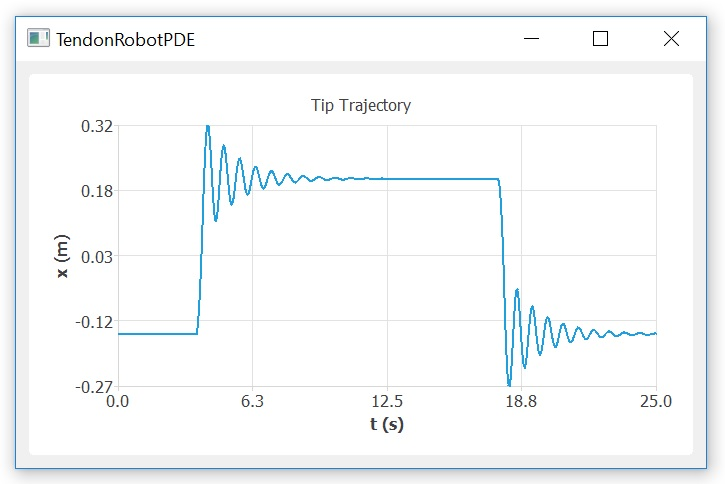
\includegraphics[width=0.6\textwidth]{fig/SolutionPlot.jpg}
	\label{fig:Plot}
\end{figure}
The damping behavior is not exactly what we would observe from a real robot since we have not modeled friction on the tendon, but we've done enough for this example.

The file ``Tendon\_Robot\_Animation.blend'' contains a script to generate an animation of the robot from the files ``centerline.dat'', ``tendon.dat'', and ``disks.dat''. The tendon motion is illustrated as prismatic for convenience.

\begin{figure}[h]
	\centering
		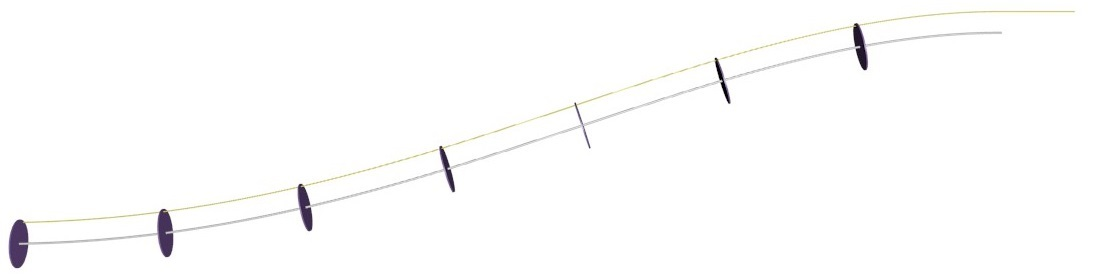
\includegraphics[width=0.95\textwidth]{fig/Render.jpg}
	\label{fig:Render}
\end{figure}

\end{document}